%%%%%%%%%%%%%%%%%%%%%%%%%%%%%%%%%%%%%%%%%%%%%%%%%%%
% emphyiscs.tex
%%%%%%%%%%%%%%%%%%%%%%%%%%%%%%%%%%%%%%%%%%%%%%%%%%%
\subsection{\textbf{Electromagnetic physics}}\label{sec:emphys}
The \Gfour{} set of electromagnetic (EM) physics processes and models 
\cite{bib:G4,bib:uni,embib:design} are used in practically all types of
simulation applications including high energy and nuclear physics experiments,
beam transport, medical physics, cosmic ray interactions and radiation effects
in space.  In addition to models for low and high energy EM physics for 
simulation of radiation effects in media, a sub-library of very low energy 
models was developed within the framework of the \Gfour{}-DNA project, with the
goal of simulating radiation effects involving physics and chemistry at the 
sub-cellular level \cite{embib:dna3}.

\subsubsection{Unification of EM physics sub-packages}\label{sec:em1} % JMCB Feedback
% Author: Omrane Kadri
%%%%%%%%%%%%%%%%%%%%%%%%%%%%%%%%%%%%%%%%%%%%%%%%%%%
% uni.tex
%%%%%%%%%%%%%%%%%%%%%%%%%%%%%%%%%%%%%%%%%%%%%%%%%%%
In the early stages of \Gfour{}, low and high energy electromagnetic processes
were developed independently, with the result that these processes could not
be used in the same run.  To resolve this problem, the interfaces were unified
so that the standard, muon, high energy, low energy and DNA EM physics 
sub-packages \cite{bib:uni} now follow the same design.

All \Gfour{} physical processes, including transportation, decay, EM, hadronic,
optical and others, were implemented via the unique general interface
\gclass{G4VProcess}.  Three EM process interfaces inherit from it via the 
intermediate classes \gclass{G4VContinuousDiscreteProcess} or 
\gclass{G4VDiscreteProcess} \cite{embib:design}:
\begin{itemize}
\item \gclass{G4VEnergyLossProcess}, which is active along the step and post
              step,
\item \gclass{G4VMultipleScattering}, which is active along the step and
\item \gclass{G4VEmProcess}, which has no energy loss and is active post step
              and at rest. 
\end{itemize}
These three base classes are responsible for interfacing to the \Gfour{} kernel, 
initializing the electromagnetic physics, managing the energy loss, range and 
cross sections tables, managing the electromagnetic models, and the built-in 
biasing options.  Each process inherits from one of these base classes, and has
one or more physics models.  EM physics models were implemented via the 
\gclass{G4VEmModel} interface.  A model is applied for a defined energy range 
and \gclass{G4Region}, allowing, for example, one model from the low energy and 
one from the high energy sub-package to be assigned to a process for a given 
particle type.

Migration to this common design resulted in an improvement of overall CPU 
performance, and made it possible to provide several helper classes which are 
useful for a variety of user applications:
\begin{itemize}
\item \gclass{G4EmCalculator}: accesses or computes cross section, energy loss,
              and range;
\item \gclass{G4EmConfigurator}: adds extra physics models per particle type, 
              energy, and geometry region; 
\item \gclass{G4EmSaturation}: adds Birks saturation of visible energy in
              sensitive detectors;
\item \gclass{G4ElectronIonPair}: samples ionization clusters in tracking
              devices.
\end{itemize}

These common interfaces enabled the full migration of EM classes to
multithreading \cite{embib:chep14} with only minor modifications of the existing
physics model codes.  Initialization of the energy loss, stopping power and 
cross section tables is carried out only once in the master thread at the
beginning of simulation and these tables are shared between threads at run time. 

Further improvements were made through the factorization of secondary energy and
angle sampling.  The \gclass{G4VEmAngularDistribution} common interface allows
the reuse of angular generator code by models in all EM sub-packages.  The
implementation of a unified interface for atomic deexcitation, 
\gclass{G4VAtomDeexcitation} provides the possibility of sampling atomic 
deexcitation by models from all EM sub-packages.
 
The consolidation of the EM sub-packages boosts the development of new models,
% and automatically resolves a number of problems seen in previous versions.
% Moreover, it 
provides new opportunities for the simulation of complex high energy and low 
energy effects and enables better validation of EM physics \cite{embib:uni2}. 

\label{sec:emuni}

\subsubsection{Gamma models}\label{sec:em2} %JMCB Feedback
% Author: Jeremy Brown
%%%%%%%%%%%%%%%%%%%%%%%%%%%%%%%%%%%%%%%%%%%%%%%%%%%
% gamma.tex 
% Coordinator J. M. C. Brown
%%%%%%%%%%%%%%%%%%%%%%%%%%%%%%%%%%%%%%%%%%%%%%%%%%%
% \begin{figure}
% 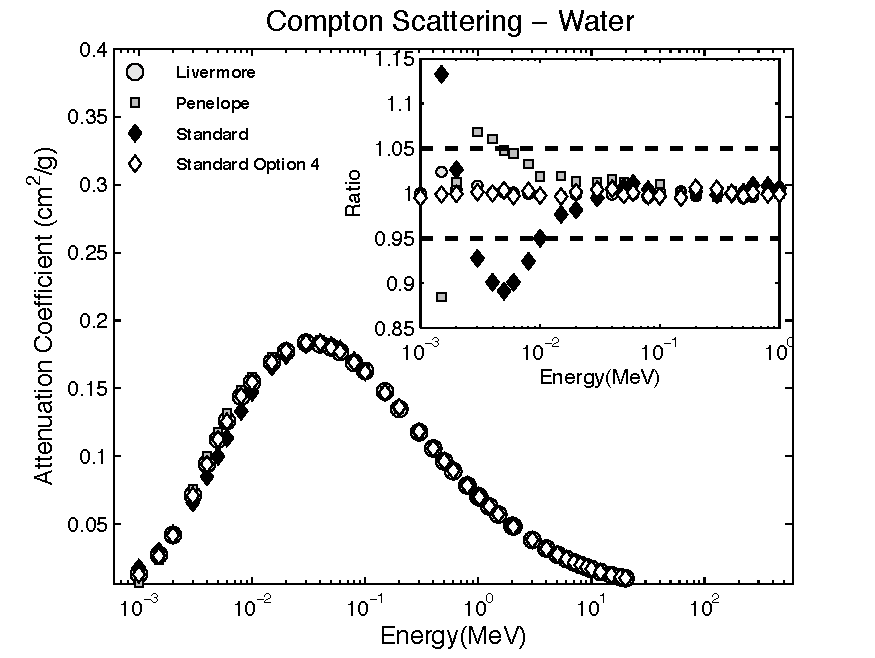
\includegraphics[width=0.5\textwidth]{figures/plot_compton.pdf}
% \caption{Compton scattering attenuation coefficient, calculated for different
%          \Gfour{} models. \gclass{G4LowEPComptonModel} is used in the Option4
%          EM physics configuration.  The inset shows the ratio of the coefficient
%          calculated using each alternative \Gfour{} electromagnetic physics list,
%          to the value from NIST XCOM \cite{embib:gamma16}.  The 
%          dashed lines correspond to a $\pm 5$\% difference.}
% \label{em:compton}
% \end{figure}
The basic set of gamma models in the EM physics packages includes models
developed for HEP applications \cite{bib:G4}, models based on the Livermore
evaluated data library \cite{embib:epdl} and a C++ implementation of the 
Penelope 2008 model \cite{embib:pen}.  Recent releases of \Gfour{} have included
revised versions of existing models, and the addition of new gamma physics 
processes and models. The low and high energy models were improved and display
similar accuracy in their shared domain of validity \cite{embib:uni2}. 
These modifications not only increased model accuracy but increased 
computational efficiency and enabled sharing of internal physics tables, 
where possible, in MT mode \cite{embib:chep14}.  
New gamma models were added to take into account physics effects not available
previously in \Gfour{} or in other simulation codes. 

A new relativistic pair production model, 
\gclass{G4Pair\allowbreak{}Production\allowbreak{}RelModel}, was developed for
simulations in astrophysics, 
LHC experiments, and other HEP applications.  This model takes into account 
the Landau-Pomeranchuk-Migdal (LPM) effect \cite{embib:gamma5}, which describes
the decrease of pair production cross sections at ultra-relativistic energies 
for dense media \cite{embib:gamma6}.  This model is physically accurate only
above 100 MeV, as no lower energy corrections are included.  It is suggested for
use in HEP applications above 80 GeV.  The use of the relativistic model is 
essential for the accurate simulation of new physics at LHC.

Two new gamma conversion models were developed to take into account the effect
of gamma ray polarization:
\begin{itemize}
\item \gclass{G4LivermorePolarized\allowbreak{}GammaConversionModel} and
\item \gclass{G4BoldyshevTripletModel} (to be used in unison with
      \gclass{G4Livermore\allowbreak{}NuclearGamma\allowbreak{}ConversionModel}).
\end{itemize}
The first is responsible for sampling electron-positron pair production by 
linearly polarized gamma rays with energies above 50 MeV \cite{embib:gamma11},
while the second (currently valid only above 100 MeV) simulates the pair 
production process in the electron field with the emission of an 
additional recoil electron \cite{embib:gamma12}, properly taking into account 
the so-called ``triplet'' production total cross section.

The Livermore polarized gamma conversion model is based on the Heitler cross
section, where the azimuthal distribution of the pair was obtained by 
integrating the cross section over energy and polar angles \cite{embib:gamma11}.

The Boldyshev triplet model uses Borselino diagrams to calculate the cross 
sections \cite{embib:pol3}.  Most of the recoil electrons in the Boldyshev model
have low energy, with a peak around $8/(T/mc^2)$, expressed in MeV, where $T$
is the gamma energy and $m$ is the electron rest mass.  Thus, a model for the
cross section was developed including a momentum threshold value of 1 $mc$, in
order to avoid the generation of too many very low energy recoil electrons
\cite{embib:pol4}. 

Finally, a specialized Compton scattering model 
\gclass{G4Low\allowbreak{}EPCompton\allowbreak{}Model} was 
developed \cite{embib:gamma13,embib:gamma14}.  Through the implementation of a
theoretical foundation that ensured the conservation of energy and momentum in
the relativistic impulse approximation \cite{embib:gamma15}, this model
implements energy and directional algorithms for both the scattered photon and 
ejected Compton electron developed from first principles. It was developed to 
address the limited accuracy of the Compton electron ejection algorithms present
in other low energy Compton scattering models that have been observed below
5~MeV \cite{embib:gamma14,embib:gamma7,embib:gamma8}. Figure \ref{em:compton} 
shows the comparison of different \Gfour{} Compton scattering cross sections
versus NIST evaluated data \cite{embib:gamma16} calculated with the methodology 
described in \cite{embib:gamma17}.  The \gclass{G4LowEPComptonModel} agrees with
the reference data to within
1\%, the statistical uncertainty of the simulation results.  The Penelope and 
Standard models result in differences up to 10\% with respect to the NIST data
for energies between 2 and 10~keV.  At higher energies, the differences are 
smaller and are below 1\% above 100 keV, corresponding to the statistical 
uncertainty of the simulation results.
\begin{figure}
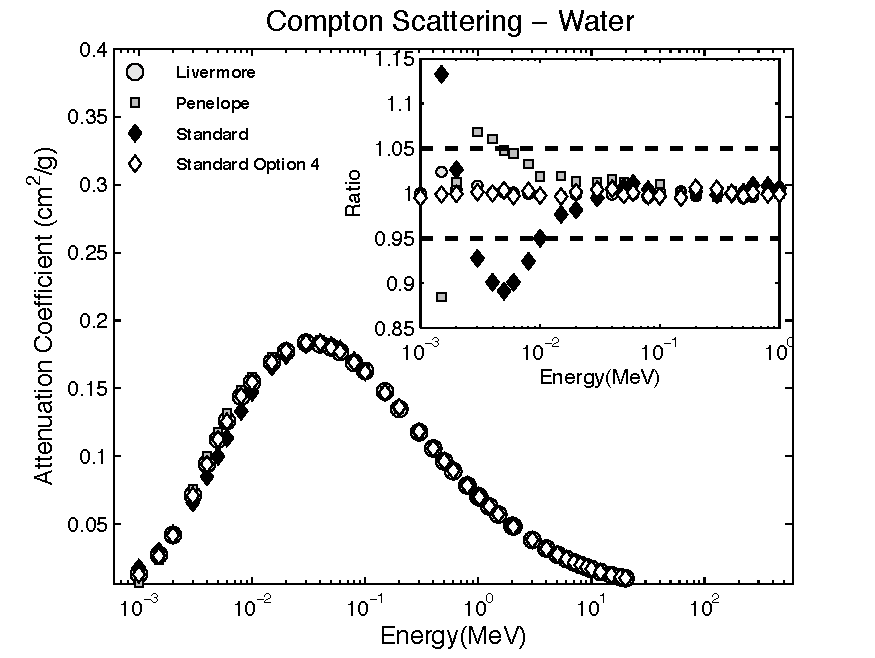
\includegraphics[width=0.5\textwidth]{figures/plot_compton.pdf}
\caption{Compton scattering attenuation coefficient, calculated for different
         \Gfour{} models. \gclass{G4LowEPComptonModel} is used in the Option4
         EM physics configuration.  The inset shows the ratio of the coefficient
         calculated using each alternative \Gfour{} electromagnetic physics list,
         to the value from NIST XCOM \cite{embib:gamma16}.  The
         dashed lines correspond to a $\pm 5$\% difference.}
\label{em:compton}
\end{figure}



\subsubsection{Ionization models}\label{sec:em3} % JMCB Feedback
% Author: Melanie Raine
%%%%%%%%%%%%%%%%%%%%%%%%%%%%%%%%%%%%%%%%%%%%%%%%%%%
% ioni.tex
%%%%%%%%%%%%%%%%%%%%%%%%%%%%%%%%%%%%%%%%%%%%%%%%%%%

\Gfour{} offers a range of ionization models for different particle types.  These 
models can be classified as either condensed or discrete.  In the condensed 
approach, the energy loss calculation has a continuous component and a discrete
one, discriminated by a given energy threshold.  Below this threshold the energy
loss is continuous, and above it the energy loss is simulated by the explicit 
production of secondary electrons \cite{embib:design}.  The user does not 
directly define the threshold because in \Gfour{} a special method of threshold 
calculations for different materials is used.  The user defines a unique 
\emph{cut in range}  \cite{bib:G4}, whose value is transformed into a kinetic 
energy threshold per material at initialization time of \Gfour{}.  Electrons 
with this kinetic energy have a mean range in a given material equal to the cut
in range and gammas have an absorption length 1/5 of the range cut.

If no value is given in the reference physics lists the default cut value of 
0.7 mm is used, providing sufficiently accurate simulation results for many 
applications.  For a specific use-case, \emph{cut in range} values should be 
optimized per geometry region.  It is recommended that this value be defined to
be less than the smallest size of geometry volumes in the region.
 
The \emph{cut in range} approach may be used for other processes besides 
ionization.  These cuts may be defined for gammas, electrons, positrons, and 
protons, and modified based on particle type and geometry region.  However, the
cut value cannot be arbitrary.  Because \Gfour{} ionization models usually have an
energy range of applicability, there is a lower limit to the electron production 
threshold.  By default the lower limit is 1 keV, but it can be changed by the 
user.  On top of this, any EM model may establish its own lower limit for the 
threshold.  If several models are applied for a given particle type, then the 
maximum of all limit values from the models is used for the particle.  For most 
ionization models the low limit is equal to the mean ionization potential of a
material. 

The list of main ionization processes and models following the condensed 
simulation approach is shown 
in Table \ref{Table-Ioni}. 
\begin{table*}
\caption{List of \Gfour{} ionization processes and models with recommended energy range.}
\label{Table-Ioni}
\begin{center}
\begin{tabular}{llll}
\hline
Particle& Process& Model& Energy range\\ \hline
 e-/e+& \gclass{G4eIonisation} & \gclass{G4MollerBhabhaModel} & 10 keV - 10 TeV\\
 e-/e+ & & \gclass{G4PenelopeIonisationModel} & 0.1 keV - 5 GeV\\
e- &  & \gclass{G4LivermoreIonisationModel} & 0.1 keV - 1 MeV \\
all & & \gclass{G4PAIModel} &   0.1 keV -  10 TeV  \\
all & & \gclass{G4PAIPhotModel} & 0.1 keV -  10 TeV \\
muons & \gclass{G4MuIonisation} & \gclass{G4BraggModel} & 0.1 keV -  0.2 MeV \\
& & \gclass{G4BetheBlochModel} & 0.2 MeV -  1 GeV \\
& & \gclass{G4MuBetheBlochModel} \cite{embib:emmu}& 1 GeV -  10 PeV \\ 
hadrons& \gclass{G4hIonisation} & \gclass{G4BraggModel} & 1 keV -  2 MeV\\
& & \gclass{G4BetheBlochModel} & 2 MeV -  10 TeV \\
& & \gclass{G4ICRU73QOModel} \cite{embib:empbar} &  5 keV -  10 MeV \\
ions & \gclass{G4ionIonisation} & \gclass{G4BraggIonModel} & (1 keV - 2 MeV)/u \\
& & \gclass{G4BetheBlochModel} & (2 MeV -  10 TeV)/u \\
 & & \gclass{G4IonParametrisedLossModel} \cite{embib:emIon}&  (1 keV - 1 GeV)/u \\
\hline
\end{tabular}
\end{center}
\end{table*}

In the condensed approach, a model of energy loss fluctuations must be used in
conjunction with the energy loss model.  The \gclass{G4VEmFluctuationModel} 
interface was developed to accommodate several implementations of fluctuation
sampling, and several models derive from it:
\begin{itemize}
\item \gclass{G4UniversalFluctuation} - default model applicable to all charged 
particles based on a previous model \cite{embib:fluc};
\item \gclass{G4IonFluctuations} -  for small steps uses
\gclass{G4UniversalFluctuation} and for big steps uses a gaussian width based
on a parameterization \cite{embib:ionfluc};
\item \gclass{G4PAIModel} and \gclass{G4PAIPhotModel} - photo-absorption 
ionization (PAI) models \cite{embib:pai}.
\end{itemize}
PAI models simultaneously provide cross sections and energy loss, and sample
energy loss fluctuations.  The ionization cross sections of the PAI models
derive from gamma absorption cross sections per atomic shell.  They are, in 
general, more accurate and stable versus simulation conditions (cuts, step 
limits, energy) than the default model \cite{embib:chep14,embib:chep11}, but are
more computationally expensive because of the internal sampling at each
ionization collision.  An illustration of simulation performance is shown in 
Figure~\ref{em:alice} for the test beam data of the ALICE Time Projection 
Chamber \cite{embib:tpc1,embib:tpc2}. 

Other studies show that PAI models generally fit the data 
independently of the step size, while the default model strongly requires the
application of extra step limitations. 

In the case of thin absorbers, the default model requires at least two particle
steps within the defined volume.  While having some difficulties for thin 
layers, the default model provides good physics performance for a variety of 
applications, in particular for tracking devices (Figure~\ref{em:silicon}), 
satisfying the requirements of most HEP experiments.

\begin{figure}
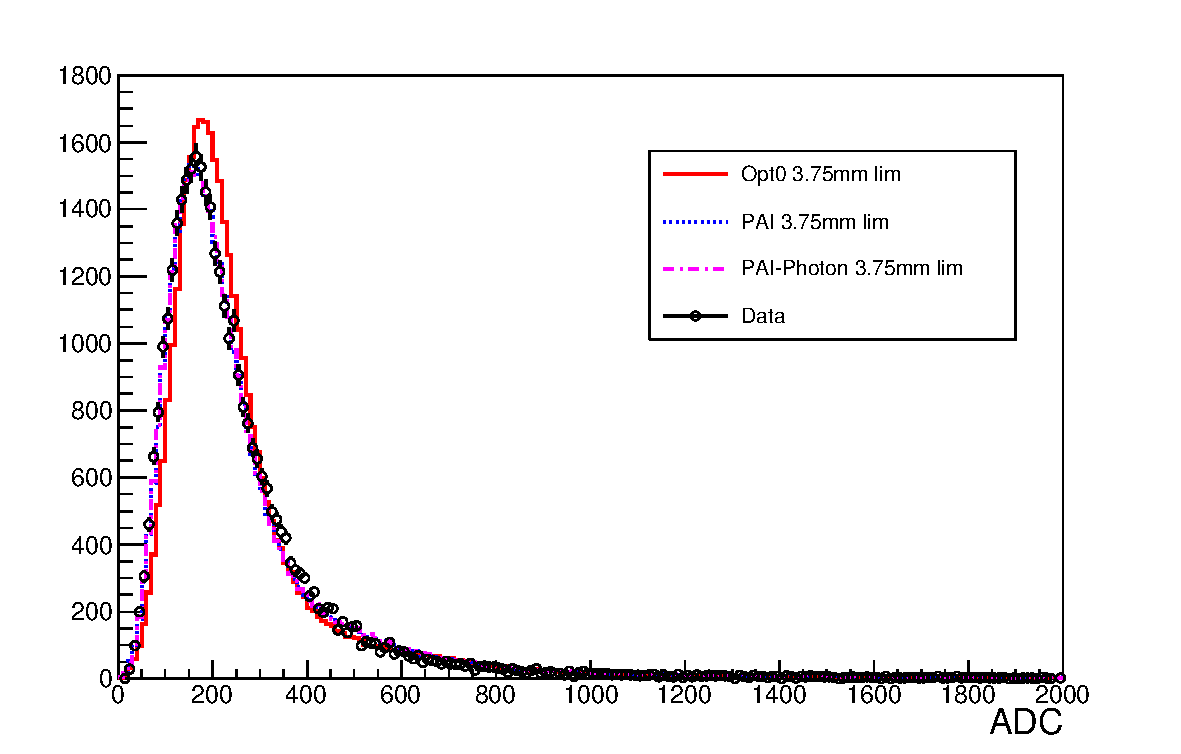
\includegraphics[width=0.5\textwidth]{figures/A_p_3gev_1mm.pdf}
\caption{Proton energy deposition in gas gap in ADC counts for a beam momentum 
         of 3 GeV/c and a gas mixture of $Ne-CO_2-N_2$.  
         The histogram represents the simulation with a 1 mm cut and a step limit
         equal to half the gap thickness.  The ADC scale for simulation was 
         normalized to the PAI model peak position.  The open circles display
         the data \cite{embib:tpc1,embib:tpc2}.}
\label{em:alice}
\end{figure}

\begin{figure}
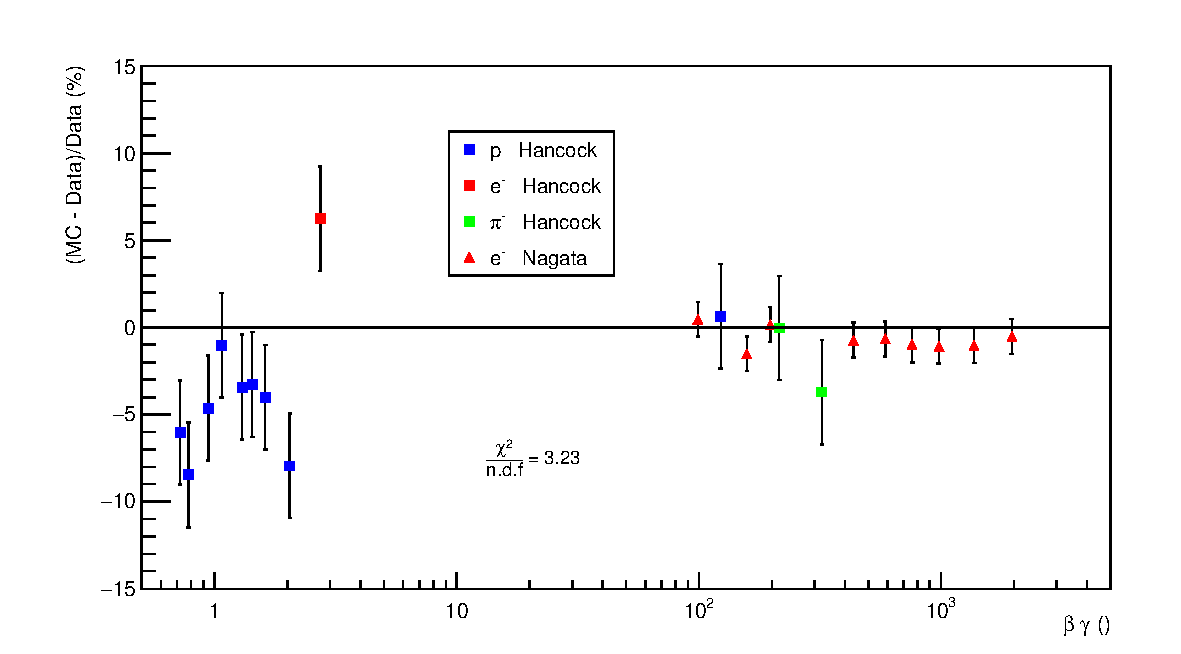
\includegraphics[width=0.5\textwidth]{figures/BetaGamma_Delta_diff_opt0_10um.pdf}
\caption{\Gfour{} versus data comparison of the most probable energy deposition in 
         thin layers of silicon (thickness 300 $\mu m$ Hancock; 1565 $\mu m$ Nagata). 
         Different beam particles and energies are used from the review
         \cite{embib:bicsel}.  Results are given in percent, and the default EM 
         physics is applied with a cut in range of 100 $\mu m$.}
\label{em:silicon}
\end{figure}

\begin{figure}
% \centering
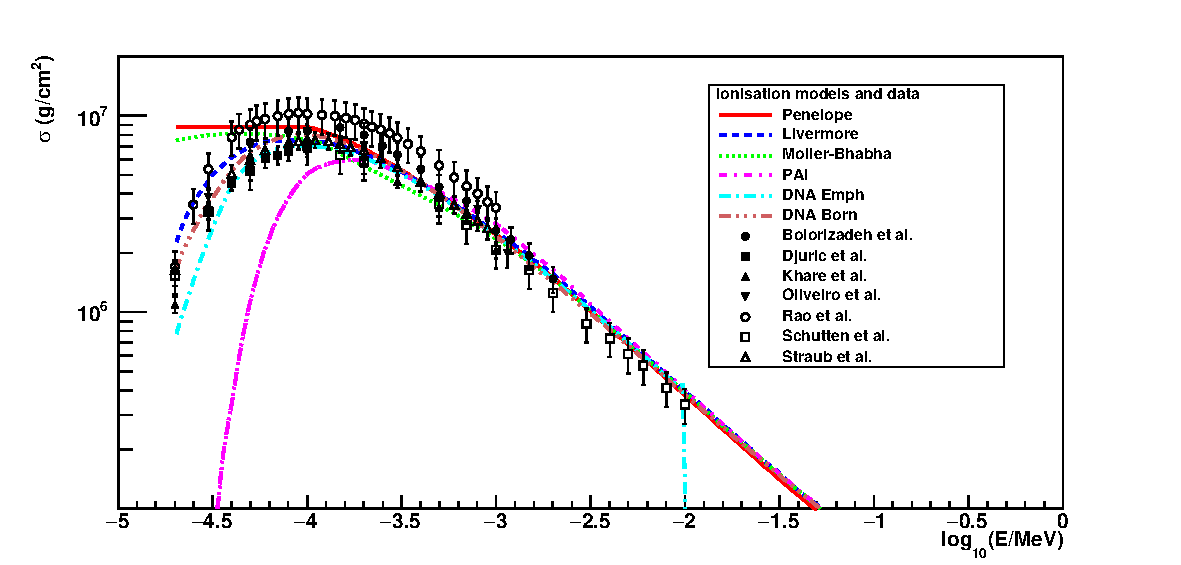
\includegraphics[width=3.8in]{figures/ApicXS_99.pdf}
\caption{Total cross section of delta electron production in liquid water as a
         function of projectile electron energy.  Curves correspond to different
         \Gfour{} ionization models, and points correspond to experimental data
         \cite{embib:dnaxs}.  The DNA model has an upper validity limit of
         1 MeV.}
\label{em:xsh2o}
\end{figure}

Recently, alternative ionization processes and models were introduced for
specific applications.  Contrary to the traditional condensed approach, these 
processes do not have a continuous energy loss component.  They explicitly 
generate all electrons down to very low energies.  They were first developed in
the framework of the \Gfour{}-DNA project (see \ref{sec:em9}), which aims to model
early biological damage induced by ionizing radiation at the DNA scale.  The 
\gclass{G4DNAIonisation} process has different models that apply to electrons, 
protons and selected ions (H, alpha, alpha+, He, Li, Be, B, C, N, O, Si and Fe)
in liquid water \cite{embib:dnaProc1, embib:dnaxs}.  Similarly, a specific
process, \gclass{G4MicroElecInelastic}, was developed for microelectronics 
applications, with a corresponding model that applies to electrons, protons and
heavy ions in silicon \cite{embib:micro, embib:micro1}.

Such models are applicable to a limited energy range and a selected set of 
materials, and in order to simulate realistic particle transport, it may be 
necessary to combine them with a continuous ionization process.  For this 
purpose the user may configure, for a given process and particle type,
several models for different energy ranges and detector regions \cite{bib:uni}.
These discrete models produce secondary electrons without the low energy 
threshold used by continuous ionization models, which could lead to 
discontinuous transitions between models.  To remedy this, the production of 
secondary electrons below the threshold may be enabled using the 
\gclass{G4VSubCutProsessor} interface, which works in parallel with the 
continuous model.

To illustrate this, cross sections of electrons in liquid water are shown in
Figure \ref{em:xsh2o}.  For the condensed approach models, a delta electron 
production threshold of 1 keV was used and the total electron cross section was
corrected for delta electron production below this threshold.



\subsubsection{Multiple and single scattering}\label{sec:em4} % JMCB Feedback
% Author: Omrane Kadri
%%%%%%%%%%%%%%%%%%%%%%%%%%%%%%%%%%%%%%%%%%%%%%%%%%%
% msc.tex
%%%%%%%%%%%%%%%%%%%%%%%%%%%%%%%%%%%%%%%%%%%%%%%%%%%
At present, the Monte Carlo simulation of charged particle transport in detailed
(interaction by interaction) mode is feasible only for projectiles with 
relatively low energies and for thin targets.  In general, the number of 
elastic interactions of a projectile before being stopped is very large and
detailed simulation becomes impractical.  The conventional solution for 
overcoming this difficulty is the implementation of condensed-history 
simulation schemes, in which the cumulative effect of many elastic scatterings
along a given track segment is simulated by using multiple scattering theories
such as Moli\`{e}re \cite{embib:msc2, embib:msc3}, Goudsmit and Saunderson
\cite{embib:msc4} and Lewis \cite{embib:msc6}.

\Gfour{} offers a diverse set of multiple scattering and single scattering
models \cite{embib:msc61,embib:msc1,embib:msc8,embib:msc9}.  Multiple scattering
models share the same \gclass{G4VMscModel} interface and were tuned per particle
type and application domain.  Recently, the possibility of sampling the lateral 
displacement of a charged particle at a geometry boundary was achieved by moving
the sampling of particle scattering from post-step to along-step, before 
sampling the energy loss and straggling.

Single scattering models sample each elastic collision of a charged particle, 
resulting in an increased number of steps and increased simulation time in 
comparison to multiple scattering models.  However, single scattering models 
have several important applications.  In particular, they are needed for the 
simulation of recoils \cite{embib:msc8,embib:msc9}, which is crucial, for 
example, for the understanding of single event effects in space electronics. 
Single scattering models are also needed to perform comparisons and validations
of multiple scattering models.  Single scattering models are useful for the 
sampling of charged particle transport in thin layers or low density media, and
in the vicinity of boundary crossing between two volumes.  In the majority of 
benchmark results for all particle types, single scattering predictions are 
closer to reference data than those of multiple scattering.

The choice of multiple scattering model strongly influences the CPU 
performance of the EM simulation.  The new unified design \cite{bib:uni} allows 
different multiple scattering models for different energy ranges to be used 
within the same simulation.  The analysis of all available results from multiple
scattering benchmarks \cite{embib:chep11,embib:msc1,embib:chep12} 
allows establishment of the optimal configuration of multiple and single 
scattering models in production physics lists.

In default physics lists, the Urban model is used below 100 MeV for electrons 
and positrons, where this model has a significant advantage in accuracy and 
CPU speed.  In the combined model \gclass{G4WentzelVIModel}, single scattering 
is applied only for hard scattering, which has a limited cross section, while
small angle scattering is sampled as multiple scattering \cite{embib:msc1}. 
The \gclass{G4WentzelVIModel} model provides results similar in accuracy to 
single scattering but it is much more computationally efficient.  As such, 
recent versions of \Gfour{} have this combined model set as the default for muon
and hadron transport, and for $e^{\pm}$ above 100 MeV.  Validation of multiple
scattering models for muons and hadrons are published elsewhere 
\cite{embib:chep14,embib:chep11,embib:msc1,embib:msc12}.

As an example of benchmark tests carried out, Figure~\ref{Figure-MSC1} 
illustrates the ratios of simulated to measured angular distribution widths
taken at the points where the distrubution falls to 1/e of the peak value.  The
measured data taken from literature \cite{embib:msc11} include a set of 
different target materials (Be, C, Al, Ti, Cu, Ta, Au) with an accuracy of about
1\%.  Using the \gclass{G4UrbanMscModel} of \Gfour{} release 10.0, the predicted 
angular distribution widths are close to the data with a maximum deviation not 
exceeding 3\% for both test cases of 13 and 20 MeV. 

\begin{figure}
\includegraphics[width=0.5\textwidth]{figures/ratio_13.pdf}
% \includegraphics[width=0.5\textwidth]{electromagnetic/ratio_13.eps}
\caption{The MC/data ratio of angular distribution widths measured at the 1/e
level for the Urban model of \Gfour{} 10.0.  Results are shown for a 13~MeV beam
on the target materials and thicknesses of the electron scattering benchmark
\cite{embib:msc11} .}
\label{Figure-MSC1}
\end{figure}




\subsubsection{Radiation of charged particles}\label{sec:em5}% JMCB Feedback
% Author: 
%%%%%%%%%%%%%%%%%%%%%%%%%%%%%%%%%%%%%%%%%%%%%%%%%%%
% brem.tex
%%%%%%%%%%%%%%%%%%%%%%%%%%%%%%%%%%%%%%%%%%%%%%%%%%%
A variety of models to simulate the radiation loss of charged particles are
available in the toolkit (Table~\ref{em:brem}).  Significant efforts were made
\cite{embib:chep12} to improve the description of EM shower shapes in order to
simulate accurate $H\to\gamma\gamma$ signals in the LHC detectors 
\cite{embib:Higgs1,embib:Higgs2}.  High energy EM shower profiles are sensitive 
to electron/positron bremsstrahlung spectra and angular distributions.
All \Gfour{} models of bremsstrahlung in the intermediate energy range 1~keV to
1~GeV are based on tables of differential cross sections published by Seltzer
and Berger \cite{embib:SelzBer}.  Evaluated 2-D tables are stored in the EM 
data set \gclass{G4LEDATA} and are loaded at initialization time.  The 
Ter-Mikaelian suppression of low energy gamma emission due to finite formation 
length (see \cite{embib:bremfl} and references therein) is taken into account 
by all models. 

\begin{table*}
\caption{List of \Gfour{} models for simulation of radiation loss with 
         recommended energy ranges. Array size refers to the internal table
         storing number of primary energy points versus number of secondary 
         energy points.}
\label{em:brem}
\begin{center}
\begin{tabular}{llll}
\hline
Particle& Model& Energy range&Array size \\ \hline
 e-/e+& \gclass{G4SeltzerBergerModel} \cite{embib:chep12}& 1 keV - 10 GeV & 57x32\\
 e-/e+ & \gclass{G4PenelopeBremsstrahlungModel} & 1 keV - 10 GeV & 57x32\\
e-  & \gclass{G4LivermoreBremsstrahlungModel} & 1 keV - 10 GeV & 31x14 \\
 e-/e+ & \gclass{G4eBremsstrahlungRelModel} \cite{embib:chep12}&   1 GeV - 10 PeV &  \\
$\mu^{\pm}$    & \gclass{G4MuBremsstrahlungModel} \cite{embib:emmu}& 1 GeV - 10 PeV & \\
$\mu^{\pm}$    & \gclass{G4MuPairProductionModel} \cite{embib:emmu}& 1 GeV - 10 PeV & 17x1000\\
$\pi^{\pm}, K^{\pm}, p$ &\gclass{G4hBremsstrahlungModel} \cite{embib:hb}&5 GeV - 10 PeV &\\
$\pi^{\pm}, K^{\pm}, p$ &\gclass{G4hPairProductionModel} \cite{embib:hb}&5 GeV - 10 PeV &13x1000 \\
\hline
\end{tabular}
\end{center}
\end{table*}
For $e^{\pm}$ above 1~GeV, a relativistic model \cite{embib:chep12} was developed
with an improved treatment of the LPM effect \cite{embib:migdal}.  This was 
implemented on top of the classical Bethe-Heitler cross section with complete 
screening.  Two types of saturation effects, LPM and formation length, have been 
combined to limit the number of low energy photons produced.  These corrections
have a distinct impact on EM shower shape and fluctuations of energy loss for
high energy EM particles, of particular importance in LHC experiments.

Because simulation of radiation losses of muons is also important for LHC 
experiments, muon bremsstrahlung and pair production models were developed
\cite{embib:emmu}.  The effect of catastrophic energy loss by high energy muon 
bremsstrahlung is well reproduced by simulation and is essential for muon 
identification.  The process of $e^+e^-$ pair production by muons dominates the
average energy loss at high energy \cite{embib:emmu}; proper simulation of the 
final state requires keeping a detailed 2-D internal table of differential cross
sections (Table~\ref{em:brem}) with a structure chosen to achieve a compromise 
between memory usage, initialization time, and accuracy \cite{embib:chep14}.  
Analysis of CMS test beam data \cite{embib:cmstb} indicates that bremsstrahlung
and pair production by pions and protons should be taken into account.  This was
achieved on top of the muon processes by changing the spin term and the mass of 
projectile particles \cite{embib:hb}. 


\subsubsection{Polarization models}\label{sec:em6} % JMCB Feedback
% Author: Paul Gueye
%%%%%%%%%%%%%%%%%%%%%%%%%%%%%%%%%%%%%%%%%%%%%%%%%%%
% polar.tex
%%%%%%%%%%%%%%%%%%%%%%%%%%%%%%%%%%%%%%%%%%%%%%%%%%%
Models for the simulation of linear polarized gamma transport are based 
on the set of Livermore gamma models: photoelectric effect \cite{embib:gamma9}, 
Rayleigh and Compton scattering \cite{embib:gamma10}, and gamma conversion. 
These models have been part of \Gfour{} for a long time.  New gamma conversion
models briefly described in Section \ref{sec:em2} also take into account linear
polarization of a primary gamma.  Also the process of positron annihilation was
updated, and now takes into account the correlation of photon polarization in 
the annihilation rest frame.

In parallel, a polarization sub-library was designed to use the standard 
gamma models \cite{embib:pol5}.  This library allows for the simulation of 
circularly polarized electrons and positrons in vacuum and in polarized media.
For a complete simulation of a low energy polarimeter setup, all processes
relevant to tracking polarized particles through matter, such as spin-dependent
Compton scattering, Bhabha-M\"{o}ller scattering, annihilation, bremsstrahlung
and pair production, were implemented.  The main application of this library is
in the design of positron sources for future linear colliders \cite{embib:pol6}.


\subsubsection{High energy models}\label{sec:em61} % JMCB Feedback 
% Author: 
%%%%%%%%%%%%%%%%%%%%%%%%%%%%%%%%%%%%%%%%%%%%%%%%%%%
% high.tex
%%%%%%%%%%%%%%%%%%%%%%%%%%%%%%%%%%%%%%%%%%%%%%%%%%%
% For specific studies at the LHC and design of future linear colliders 
% \cite{embib:lin}, a set of high energy models have been developed. 
The processes of gamma conversion to muon pairs \cite{embib:gmumu}, and positron
annihilation into muons and hadrons \cite{embib:emmu}, were implemented to assist
in the design of interaction regions within future linear colliders
\cite{embib:lind}.  Other models were added for the simulation of energy loss of
heavy exotic particles, in particular, magnetic monopoles \cite{embib:empbar}. 
Because the charges and masses of these objects are not always defined, the new 
models allow for the flexible definition of the energy ranges over which they
are valid, and are not constrained by the lower or upper limits seen in Table
\ref{Table-Ioni}.  An efficient generator for synchrotron radiation by 
relativistic electrons in magnetic fields was also implemented \cite{embib:syn}
and recently generalized to synchrotron radiation for any type of long-lived 
charged particle.



\subsubsection{Atomic de-excitation}\label{sec:em7} % JMCB Feedback 
% Author: 
%%%%%%%%%%%%%%%%%%%%%%%%%%%%%%%%%%%%%%%%%%%%%%%%%%%
% deex.tex
%%%%%%%%%%%%%%%%%%%%%%%%%%%%%%%%%%%%%%%%%%%%%%%%%%%

Atomic de-excitation can be activated in all EM physics lists through the common
atomic de-excitation interface \gclass{G4VAtomDeexcitation} \cite{bib:uni}.
Photo-electric effect, Compton scattering, and discrete ionization models 
provide cross sections of ionization for each atomic shell.  The de-excitation
code is responsible for sampling the electromagnetic cascade with fluorescence
and Auger electron emission, and was implemented using evaluated data 
\cite{embib:eadl}. Recently, alternative, more accurate transition energies have
become available in \Gfour{} 10.1 through the addition of a new data set 
\cite{embib:SPaltani}.

The ionization cross section model for Particle Induced X-ray Emission (PIXE) is
based on the condensed history approach.  Specific cross sections can be defined
for electrons, protons, and ions.  Users can select from different sets of 
theoretical or empirical shell ionization cross sections \cite{embib:pixe}.

The simulation of K, L, and M X-ray yields demands knowledge of the X-ray 
production cross sections.  These were calculated using the ECPSSR theory, 
initially developed by Brandt and Lapicki \cite{embib:deex1} and recently 
reviewed \cite{embib:deex2,embib:deex3}.  Computing the X-ray production cross 
sections from first principles is a time-consuming process due to the numerical 
double integral of form factor functions needed to obtain the ionization cross 
sections for each shell or sub-shell (Eq.(23) of \cite{embib:deex2}), over all 
possible values of the energy and momentum transfer of the incident particle.  

The calculation was expedited through the use either of extensive tables and
interpolation methods, or efficient algorithms providing sufficiently good
approximations.
% Aside from empirical tabulations data and a full analytical
% calculations method, efficient algorithms were implemented to determine K, L 
% and M-shells ionization cross-sections
% for H and He ions. 
Algorithms were implemented based on the ECPSSR ionization cross sections for
H and He ions calculated for the K and L shells using the form factor functions
for elements with atomic number 6 to 92 over the energy range of 0.1 to 100 
MeV.  In the case of the M shells, the ionization cross sections are given 
for elements with atomic number 62 to 92 over the energy range of 0.1 to 10 MeV.
Furthermore, the tables generated to develop the algorithms were obtained by
the integration of the form factor functions that describe the process using 
Lobatto's rule \cite{embib:deex4}, and are also available.  The cross sections
generated by the algorithms deviate less than 3\% from the tabulated values, 
roughly matching the scatter of empirical data \cite{embib:deex2}.  Further 
details and considerations of these calculations can be found in 
\cite{embib:deex2,embib:deex3}.  Comparisons of simulated and experimental 
spectra obtained under proton irradiation of several materials are shown in
\cite{embib:deex5,embib:deex6}.



\subsubsection{Optical physics}\label{sec:em8} % JMCB Feedback 
% Author: Peter Gumplinger
%%%%%%%%%%%%%%%%%%%%%%%%%%%%%%%%%%%%%%%%%%%%%%%%%%%
% xray_opt.tex
%%%%%%%%%%%%%%%%%%%%%%%%%%%%%%%%%%%%%%%%%%%%%%%%%%%
\Gfour{} can accurately simulate nonlinear scintillators where the light yield is
a function of particle type, energy deposition and kinetic energy of the 
ionizing particle \cite{em:opt1}.  In scintillators with a linear response, 
light production is directly proportional to the ionizing energy deposited and
the total light produced can be computed as the sum of the light produced during
small simulation steps without regard for the kinetic energy of the ionizing 
particle at each energy-depositing step.

In scintillators with a nonlinear response, the yield during a step is
calculated as the difference in yields for hypothetical, totally absorbed 
particles at the kinetic energies before and after the step.  This method 
correctly models the total light produced by a multiple step ionizing particle 
track, and accounts for two important cases.  In the first case, light is 
produced correctly for incomplete energy deposition of a charged particle, such
as when the particle exits the scintillator volume or when the particle is 
absorbed in a nuclear reaction.  In the second case, the scintillation photon 
density is larger in the high kinetic energy portion of the track for the usual
case where the nonlinear photon yield increases with particle energy.  This 
enables the precision simulation of organic or noble gas scintillators, provided
the user supplies the required data inputs.

Two more refinements in the generation of optical photons are that the 
scintillation process takes into account a finite light emission rise-time, 
and that the Cerenkov photon origin density along the track segment is no longer 
constant, but assumes a linear decrease in the mean number of photons generated 
over the step as the radiating particle slows down.

For the propagation of optical photons, the reflectivity from a metal surface
may now be calculated by using a complex index of refraction \cite{embib:Iowa}.
%\footnote{Thanks to Sehwook Lee and John Hauptman (Iowa State 
%University)} 
Mie scattering was added following the \mbox{Henyey-Greenstein} approximation, 
with the forward and backward angles treated separately \cite{embib:Mie}.
% \footnote{Thanks to Xin Qian (Caltech) based on work from Vlasios 
% Vasileiou (University of Maryland)} 
Surface reflections may be simulated using look-up tables containing measured
optical reflectance for a variety of surface treatments \cite{em:opt2}. It is 
possible to define anti-reflective coatings, and transmission of a dichroic 
filter where the transmission, or conversely the reflection, is dependent on 
wavelength and incident angle.  The optical boundary process also works in 
situations where the surface is between two volumes, each defined in a different
parallel world, thus allowing optical photon propagation for previously 
impossible geometry implementations.

%end


\subsubsection{\Gfour{}-DNA physics models}\label{sec:em9} % JMCB Feedback 
% Author: Sebastien Incerti
%%%%%%%%%%%%%%%%%%%%%%%%%%%%%%%%%%%%%%%%%%%%%%%%%%%
% dna.tex
%%%%%%%%%%%%%%%%%%%%%%%%%%%%%%%%%%%%%%%%%%%%%%%%%%%
\Gfour{} offers a set of physics processes and models \cite{embib:dna0} to 
simulate track structure in liquid water, the main component of biological
media.  These were developed as part of the \Gfour{}-DNA project 
\cite{embib:dnaweb}, and extend  
% in 2001 by the European 
% Space Agency 
\Gfour{} to include the simulation of biological damage by ionizing radiation
\cite{embib:dna1,embib:dna2}. 

The first set of discrete processes was delivered in 2007 \cite{embib:dnaProc1}.
Their accuracy was further evaluated and improved 
\cite{embib:dnaxs, embib:dnaProc2, embib:dnaProc3} through the inclusion, 
for example, of more accurate modeling of electron elastic scattering
\cite{embib:dnaElast}, and additional physical processes for sub-excitation
electrons, such as vibrational excitation and molecular attachment 
\cite{embib:dnaTS}.  These processes are critical for the modeling of
physico-chemical processes in liquid water \cite{embib:chem:paper1}. 

A major design upgrade of the software classes was applied in order to allow 
their combination with other \Gfour{} EM processes and models, for a coherent 
modeling of EM interactions \cite{bib:uni,embib:dnaPhysList}.  Thus, for 
their simulation applications, users may instantiate a 
\gclass{G4EmDNA\allowbreak{}Physics} object from their physics list.  This 
physics constructor contains all required \Gfour{}-DNA physics processes and 
models for
\begin{itemize} 
\item electrons, including ionization, excitation, elastic scattering, 
      vibrational excitation and attachment,
\item protons and neutral hydrogen, including excitation, ionization, electron
      capture and stripping,
\item alpha particles and their charged states, including excitation,
      ionization, electron capture and stripping, and  
\item ionization for Li, Be, B, C, N, O, Si and Fe ions.
\end{itemize}
 
Stopping powers and ranges simulated with \Gfour{}-DNA have been compared to
international recommendations \cite{embib:dnaStop}.  These processes can be
combined with \Gfour{} gamma processes.  Note that the \emph{Livermore} low
energy electromagnetic gamma models are selected by default in the 
\gclass{G4EmDNA\allowbreak{}Physics} constructor. 

As an illustration, \\
\verb"examples/extended/medical/dna/dnaphysics"\\
explains how to use this physics constructor.  In addition,
\verb"examples/extended/medical/dna/microdosimetry" describes how to 
combine \Gfour{}-DNA and \Gfour{} standard electromagnetic processes in a simple
user application.  A variety of applications based on \Gfour{}-DNA processes and
models allow the study of elementary energy deposition patterns at the 
sub-cellular scale.  For example, the comparison of dose point kernels 
\cite{embib:dnaPK}, $S$-values  \cite{embib:dnaS}, radial doses 
\cite{embib:dnaRad}, cluster patterns for ions with the same LET 
\cite{embib:dnaLET}, the effect of a magnetic field on electron track structures
\cite{embib:dnaMag}, and the modeling of direct DNA damage 
\cite{embib:dnaDirD1,embib:dnaDirD2,embib:dnaDirD3,embib:dnaDirD4}
have so far been explored utilizing these tools.  They even provide a framework
for the future study of non-targeted biological effects \cite{embib:dnaBio}, 
extending further the first applications of \Gfour{} electromagnetic physics at 
the physics-biology frontier
\cite{embib:dnaBio1,embib:dnaBio2,embib:dnaBio3,embib:dnaBio4,embib:dnaBio6,embib:dnaBio7,embib:dnaBio8}.



\subsubsection{\Gfour{}-DNA physico-chemistry module}\label{sec:em10} % JMCB Feedback 
% Author: Mathieu Karamitros
%%%%%%%%%%%%%%%%%%%%%%%%%%%%%%%%%%%%%%%%%%%%%%%%%%%
% chem.tex
%%%%%%%%%%%%%%%%%%%%%%%%%%%%%%%%%%%%%%%%%%%%%%%%%%%

Radiation chemistry is the science of the chemical effects of radiation on
matter.  Simulation tools in this field are relevant to many applications, such
as the production of polymers by the irradiation of monomers.  However, one of
the most studied materials under irradiation is liquid water, because it is used
as a coolant in nuclear power plants and its irradiation may create oxidative 
species that are likely to initiate the corrosion process.  Water is also of 
interest because it is the main component of biological materials.

When biological targets are exposed to radiation, the chemical response can be 
complex, depending on the composition of the medium as well as on the energy and
type of radiation.  For example, water radiolysis (dissociation of water by 
radiation) promotes the creation of oxidative species.  These species can either
react with one another or with the biological materials, interfering with the 
normal functioning of one or many cells.

In the context of the \Gfour{}-DNA project, a prototype for simulating radiation 
chemistry was developed \cite{embib:dna3, embib:chem:paper1} and delivered with
\Gfour{} version 10.1.  It is now possible to simulate the physical stage, the 
physico-chemical stage (lasting up to about 1 picosecond) and the chemical stage
(from 1 picosecond up to 1 microsecond) of water radiolysis.
%   The simulation proceeds in two stages, the first 
% consisting of prompt physics processes (reaction times $ < 10^{-9} s$) which 
% provide a set of wounded biological and water molecules in a volume of interest, 
% and the second consisting of physico-chemical processes with reaction times up
% to $10^{-6} s$. 

The \Gfour{}-DNA physical processes may in some cases create
water molecules which are electronically modified, that is, they may be ionized,
excited or have extra electrons in the case of dissociative attachment.  The 
electronic and atomic readjustment of the water molecules can eventually lead to
their dissociation.  The dissociation of water molecules is taken into account 
by random selection using user-defined branching ratios \cite{embib:chem:paper1}.
The positioning of the dissociative products is defined by the 
\gclass{G4DNAWater\allowbreak{}DissociationDisplacer} class from qualitative 
considerations \cite{embib:chem:Kreipl2009}.  It is assumed that the 
dissociation of water molecules is independent of the physical stage of the 
simulation.  This is to say that only electronic modifications undergone by the
water molecule are responsible for the dissociative pathways.  The branching 
ratios and positioning of dissociative products may be adjusted by the user if 
necessary.

Dissociative products can recombine to form new chemical species. To take this 
recombination into account, a stepping algorithm was developed specifically for 
managing collisions between \Gfour{} tracks.  The purpose of this algorithm is 
to synchronize the transport of tracks during simulation.  This means that all 
tracks are transported over the same time, accounting for chemical reactions 
that may happen during a given time step. A description of this synchronized 
stepping, applied to radiation chemistry, is available 
in \cite{embib:dna3,embib:chem:these}.

This stepping mechanism could, in principle, be applied to applications other
than radiation chemistry.  A process must first be made compatible with the 
\gclass{G4VITProcess} interface, which contains track information.  To run a 
radio-chemistry simulation, a table of reactions describing the supported 
reactions and the corresponding reaction rates must be provided.

To simplify the use of the chemistry module, the 
\gclass{G4EmDNA\allowbreak{}Chemistry} constructor provides default settings,
and three examples, 
\verb"examples/extended/medical/dna/chem1", 
\verb"examples/extended/medical/dna/chem2" and
\verb"examples/extended/medical/dna/chem3", are included.  These examples 
progressively demonstrate how to activate and use the chemistry module from a
user application. The module may be used with or without irradiation.

The chemistry module is compatible with the current event-level multithreaded 
mode of \Gfour{}.  However, the use of the module in this mode with a large number
of simulated objects or threads is not recommended because synchronized stepping
requires intense memory usage.

For now, the chemistry module allows prediction of the chemical kinetics induced 
by ionizing radiation. A future goal of the \Gfour{}-DNA project is to account for
DNA damage resulting from irradiation. 


% % \subsubsection{Physics Lists}\label{sec:em11} % JMCB Feedback 
% % Author: 
% % %%%%%%%%%%%%%%%%%%%%%%%%%%%%%%%%%%%%%%%%%%%%%%%%%%%
% phys.tex
%%%%%%%%%%%%%%%%%%%%%%%%%%%%%%%%%%%%%%%%%%%%%%%%%%%
%Many years of experience with Geant4 across a large number of applications 
%has demonstrated the significant advantage of a modular physics lists approach, 
%where each type of physics is instantiated by a \emph{physics constructor} 
%class. Geant4 maintains several EM constructors (Table~\ref{em:physl}) which 
%are created for different application domains. These constructor classes are 
%components of full Geant4 reference physics lists 
%(for example, $FTFP\_BERT$, $FTFP\_BIC\_EMY$...), and are available for EM 
%production physics constructors (names are defined in Table~\ref{em:physl}). 
%At the same time, all EM constructors may be directly used by custom 
%physics lists.

%The physics of a \Gfour\ simulation is built in a modular approach, in which a
%list (called a physics list) of interaction types is created. 

Electromagnetic physics is defined in physics constructor classes, which are
components of full physics classes. \Gfour{} maintains several EM constructors
(Table~\ref{em:physl}) for different application domains. The constructors are 
used by both \Gfour{} reference physics lists and custom physics lists.

For HEP experiments, high efficiency CPU performance is required, and, as 
such, the HEP physics configuration should provide a compromise between 
accuracy and CPU speed. For simulation of shielding in space and for radiation 
dose in medical studies, more detailed tracking of low energy particles is 
required. For this purpose, in physics constructors oriented towards medicine 
and space science applications 
(i.e. \gclass{G4EmStandardPhysics\_option4}, named $EMZ$), more strong step 
limitation are defined and models with more detailed treatment of atomic 
effects and detailed ion stopping powers are applied. A general goal is to 
provide a physics constructor with set of the most accurate models for each 
energy range and particle type.

To assist in the production and testing of physics constructors, 
experimental constructors are available. 
\Gfour{}-DNA physics constructors are applicable only 
for a limited set of materials (mainly liquid water). Examples 
of how to build physics lists with \Gfour{}-DNA physics, low energy, 
and standard 
physics \cite{embib:uni} are distributed with \Gfour{}. Specific physics 
constructors are provided for optical physics which can be added 
on top of any existing physics list.

\begin{table*}
\caption{List of \Gfour{} EM physics constructors}
\label{em:physl}
\begin{center}
\begin{tabular}{llll}
\hline
Constructor& Application& Name & Comment \\ \hline
\gclass{G4EmStandardPhysics} & HEP &  &default (ATLAS)\\
\gclass{G4EmStandardPhysics_option1} & & EMV & simplified (CMS)\\
\gclass{G4EmStandardPhysics_option2} & & EMX & simplified (LHCb)\\
\hline
\gclass{G4EmStandardPhysics_option3} & space \& & EMY & detailed  \\
                             &  medicine &     & standard models\\
\gclass{G4EmLivermorePhysics} & & LIV & detailed  \\
                     &       &          &  Livermore models\\
\gclass{G4EmPenelopePhysics} &  & PEN & detailed \\ 
                    &  &     & Penelope models\\
\gclass{G4EmStandardPhysics_option4} &  & EMZ & combining \\
                             &  &     & best models\\
\hline
\gclass{G4EmLivermorePolarizedPhysics} &  &  & polarized models\\
\gclass{G4EmLowEPPhysics} &  &  & new low energy models\\
\gclass{G4EmStandardPhysicsWVI} &  &  & WVI multiple scattering\\
\gclass{G4EmStandardPhysicsSS} &  &  & single scattering \\
\hline
\gclass{G4EmDNAPhysics} & DNA &  & default for DNA physics \\
\gclass{G4EmDNAPhysics_option1} & DNA &  & WVI multiple scattering \\
\hline
\gclass{G4OpticalPhysics} & all &  & production and transport \\
                 &     &  & of optical photons \\
\hline
\end{tabular}
\end{center}
\end{table*}


\subsubsection{Built-in EM biasing options}\label{sec:em12} % JMCB Feedback
% Author: Daren Sawkey
%%%%%%%%%%%%%%%%%%%%%%%%%%%%%%%%%%%%%%%%%%%%%%%%%%%
% bias.tex
%%%%%%%%%%%%%%%%%%%%%%%%%%%%%%%%%%%%%%%%%%%%%%%%%%%
Four biasing and variance reduction options are available within the EM
sub-libraries of \Gfour{} \cite{embib:uni2}: 
\begin{itemize}
\item cross section biasing, which may be used to study the effects of 
      uncertainties of cross sections;
\item forced interaction, implemented for the limited use-case of a thin target; 
\item splitting, where the interaction of a primary of weight $W$ which would 
      normally produce 1 secondary of weight $W$, instead produces $N$ secondaries,
      each with weight $W/N$, with no modification of the energy of the primary;
\item Russian roulette, where secondaries produced by the interaction of a
      primary particle of weight $W$ are killed with probability $1 - P$, and
      the survivors' weight is set to $W/P$; users may define $P$ and the upper 
      energy limit for secondaries for which the method is applied.
\end{itemize}

These four options are selectable through macro commands or C++ interfaces, 
and can be applied in user-defined \gclass{G4Region}s.


\subsubsection{Validation and verification of EM models}\label{sec:em13}
% Author: Vladimir Ivanchenko
%%%%%%%%%%%%%%%%%%%%%%%%%%%%%%%%%%%%%%%%%%%%%%%%%%%
% val.tex
%%%%%%%%%%%%%%%%%%%%%%%%%%%%%%%%%%%%%%%%%%%%%%%%%%%
Validation of EM physics is performed on several levels.  Because EM physics is
used in practically all tests and examples, the \Gfour{} integrated test system 
routinely checks all EM physics models.  A specific EM validation suite
\cite{embib:emVal} runs on a regular basis for each reference version of \Gfour{}
(see \cite{embib:chep14,embib:chep11,embib:chep12} and references therein).
Dedicated validations of cross sections, stopping powers, and atomic transition
energies versus evaluated data and theory are done by \Gfour{} developers and 
different user groups (see, for example, 
\cite{embib:uni2,embib:valGam,embib:valGam2} and 
Figure \ref{em:compton}).  EM physics validation is also performed in various
application domains by different user communities, especially by the HEP 
experiments ATLAS and CMS. 

As an example of EM physics validation for HEP applications, the energy 
resolution of two sampling calorimeters \cite{embib:uni3,embib:uni4} 
versus the cut in range value and \Gfour{} version is shown in 
Figure~\ref{Figure-UEM1}.  This plot illustrates the good agreement of \Gfour{}
simulation predictions with data, and the stability between \Gfour{} versions of 
simulation results for high energy physics applications.

\begin{figure}
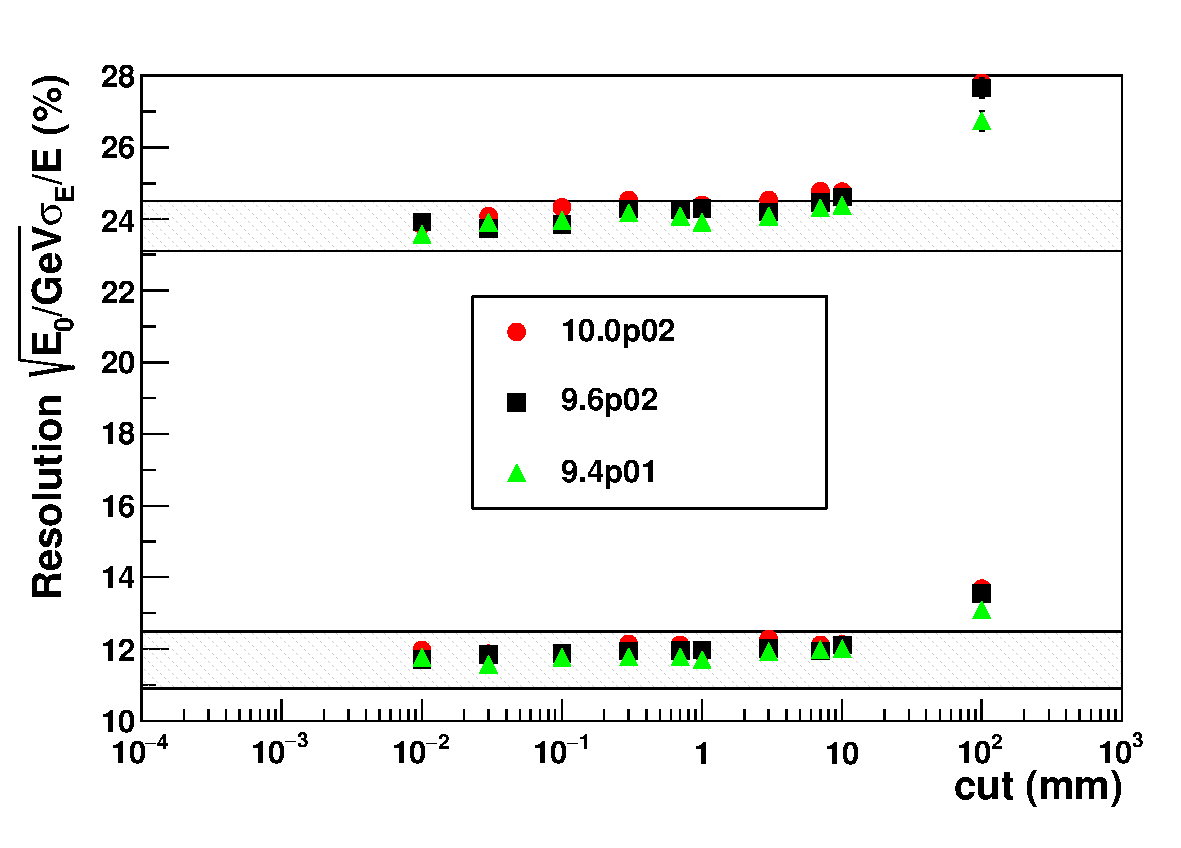
\includegraphics[width=0.5\textwidth]{figures/Azeus.pdf}
\caption{Energy resolution of two sampling Lead/Scintillator calorimeters 
for 10 GeV electrons: squares, circles and triangles indicate \Gfour{} 
simulations for different versions of the toolkit, and each band indicates 
experimental data with one standard deviation uncertainty
\cite{embib:uni3,embib:uni4}.}
\label{Figure-UEM1}
\end{figure}

Further validations come from the medical and space communities, in particular, 
GATE \cite{embib:GATE}, GAMOS \cite{embib:GAMOS}, GRAS \cite{embib:gras}, 
and TOPAS \cite{embib:TOPAS}.
There are also many validation results obtained by single user groups.  For 
example, validations for space shielding were done recently in 
\cite{embib:elshield} and for therapeutic ion beam simulation in 
\cite{embib:emIonUser}.

%end


%end
